\documentclass{article}
\usepackage[letterpaper]{geometry}
\geometry{verbose,tmargin=1in,bmargin=1in,lmargin=1in,rmargin=1in}

\usepackage[utf8]{inputenc}
\usepackage{amsmath}
\usepackage{listings}
\usepackage{graphicx}
\usepackage{enumitem}
\usepackage{amssymb}
\usepackage{tabularx}
\usepackage{hyperref}
\usepackage{caption}
\usepackage{float}
\usepackage[section]{placeins}

\title{CIS 419/519: Homework 5}
\author{Jiatong Sun}
\date{03/13/2020}

\begin{document}
    \maketitle
    \noindent
    Although the solutions are entirely my own, I consulted with the following people and sources while working on this homework: 
    
    \section{Logical Functions with Neural Nets}
        \begin{enumerate}[label=\alph*.]
            \item % a
				\begin{minipage}[t]{\linewidth}
                	\captionsetup{type=figure}
                	\centering
                	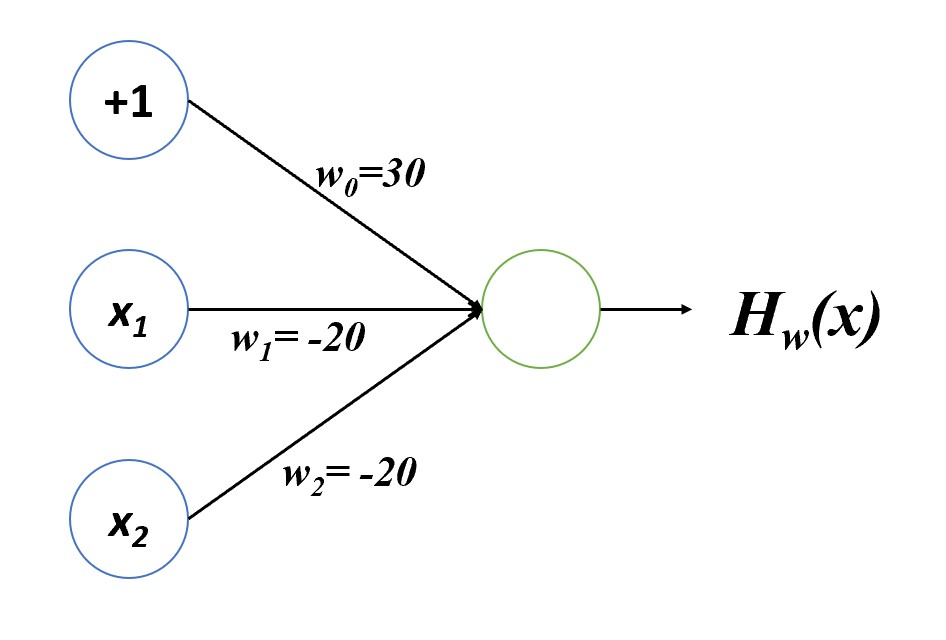
\includegraphics[width=0.6\linewidth]
                					{images/Q1a.jpg}
                	\caption{NAND}      
        		\end{minipage} 
        		
        		           
            
            \item % b
            
        \end{enumerate}
        
    \section{Calculating Backprop by Hand}
        
    \section{Neural Nets in SuperTuxKart}
       
\end{document}